% Options for packages loaded elsewhere
\PassOptionsToPackage{unicode}{hyperref}
\PassOptionsToPackage{hyphens}{url}
%
\documentclass[
]{article}
\usepackage{amsmath,amssymb}
\usepackage{iftex}
\ifPDFTeX
  \usepackage[T1]{fontenc}
  \usepackage[utf8]{inputenc}
  \usepackage{textcomp} % provide euro and other symbols
\else % if luatex or xetex
  \usepackage{unicode-math} % this also loads fontspec
  \defaultfontfeatures{Scale=MatchLowercase}
  \defaultfontfeatures[\rmfamily]{Ligatures=TeX,Scale=1}
\fi
\usepackage{lmodern}
\ifPDFTeX\else
  % xetex/luatex font selection
\fi
% Use upquote if available, for straight quotes in verbatim environments
\IfFileExists{upquote.sty}{\usepackage{upquote}}{}
\IfFileExists{microtype.sty}{% use microtype if available
  \usepackage[]{microtype}
  \UseMicrotypeSet[protrusion]{basicmath} % disable protrusion for tt fonts
}{}
\makeatletter
\@ifundefined{KOMAClassName}{% if non-KOMA class
  \IfFileExists{parskip.sty}{%
    \usepackage{parskip}
  }{% else
    \setlength{\parindent}{0pt}
    \setlength{\parskip}{6pt plus 2pt minus 1pt}}
}{% if KOMA class
  \KOMAoptions{parskip=half}}
\makeatother
\usepackage{xcolor}
\usepackage[margin=1in]{geometry}
\usepackage{color}
\usepackage{fancyvrb}
\newcommand{\VerbBar}{|}
\newcommand{\VERB}{\Verb[commandchars=\\\{\}]}
\DefineVerbatimEnvironment{Highlighting}{Verbatim}{commandchars=\\\{\}}
% Add ',fontsize=\small' for more characters per line
\usepackage{framed}
\definecolor{shadecolor}{RGB}{248,248,248}
\newenvironment{Shaded}{\begin{snugshade}}{\end{snugshade}}
\newcommand{\AlertTok}[1]{\textcolor[rgb]{0.94,0.16,0.16}{#1}}
\newcommand{\AnnotationTok}[1]{\textcolor[rgb]{0.56,0.35,0.01}{\textbf{\textit{#1}}}}
\newcommand{\AttributeTok}[1]{\textcolor[rgb]{0.13,0.29,0.53}{#1}}
\newcommand{\BaseNTok}[1]{\textcolor[rgb]{0.00,0.00,0.81}{#1}}
\newcommand{\BuiltInTok}[1]{#1}
\newcommand{\CharTok}[1]{\textcolor[rgb]{0.31,0.60,0.02}{#1}}
\newcommand{\CommentTok}[1]{\textcolor[rgb]{0.56,0.35,0.01}{\textit{#1}}}
\newcommand{\CommentVarTok}[1]{\textcolor[rgb]{0.56,0.35,0.01}{\textbf{\textit{#1}}}}
\newcommand{\ConstantTok}[1]{\textcolor[rgb]{0.56,0.35,0.01}{#1}}
\newcommand{\ControlFlowTok}[1]{\textcolor[rgb]{0.13,0.29,0.53}{\textbf{#1}}}
\newcommand{\DataTypeTok}[1]{\textcolor[rgb]{0.13,0.29,0.53}{#1}}
\newcommand{\DecValTok}[1]{\textcolor[rgb]{0.00,0.00,0.81}{#1}}
\newcommand{\DocumentationTok}[1]{\textcolor[rgb]{0.56,0.35,0.01}{\textbf{\textit{#1}}}}
\newcommand{\ErrorTok}[1]{\textcolor[rgb]{0.64,0.00,0.00}{\textbf{#1}}}
\newcommand{\ExtensionTok}[1]{#1}
\newcommand{\FloatTok}[1]{\textcolor[rgb]{0.00,0.00,0.81}{#1}}
\newcommand{\FunctionTok}[1]{\textcolor[rgb]{0.13,0.29,0.53}{\textbf{#1}}}
\newcommand{\ImportTok}[1]{#1}
\newcommand{\InformationTok}[1]{\textcolor[rgb]{0.56,0.35,0.01}{\textbf{\textit{#1}}}}
\newcommand{\KeywordTok}[1]{\textcolor[rgb]{0.13,0.29,0.53}{\textbf{#1}}}
\newcommand{\NormalTok}[1]{#1}
\newcommand{\OperatorTok}[1]{\textcolor[rgb]{0.81,0.36,0.00}{\textbf{#1}}}
\newcommand{\OtherTok}[1]{\textcolor[rgb]{0.56,0.35,0.01}{#1}}
\newcommand{\PreprocessorTok}[1]{\textcolor[rgb]{0.56,0.35,0.01}{\textit{#1}}}
\newcommand{\RegionMarkerTok}[1]{#1}
\newcommand{\SpecialCharTok}[1]{\textcolor[rgb]{0.81,0.36,0.00}{\textbf{#1}}}
\newcommand{\SpecialStringTok}[1]{\textcolor[rgb]{0.31,0.60,0.02}{#1}}
\newcommand{\StringTok}[1]{\textcolor[rgb]{0.31,0.60,0.02}{#1}}
\newcommand{\VariableTok}[1]{\textcolor[rgb]{0.00,0.00,0.00}{#1}}
\newcommand{\VerbatimStringTok}[1]{\textcolor[rgb]{0.31,0.60,0.02}{#1}}
\newcommand{\WarningTok}[1]{\textcolor[rgb]{0.56,0.35,0.01}{\textbf{\textit{#1}}}}
\usepackage{longtable,booktabs,array}
\usepackage{calc} % for calculating minipage widths
% Correct order of tables after \paragraph or \subparagraph
\usepackage{etoolbox}
\makeatletter
\patchcmd\longtable{\par}{\if@noskipsec\mbox{}\fi\par}{}{}
\makeatother
% Allow footnotes in longtable head/foot
\IfFileExists{footnotehyper.sty}{\usepackage{footnotehyper}}{\usepackage{footnote}}
\makesavenoteenv{longtable}
\usepackage{graphicx}
\makeatletter
\def\maxwidth{\ifdim\Gin@nat@width>\linewidth\linewidth\else\Gin@nat@width\fi}
\def\maxheight{\ifdim\Gin@nat@height>\textheight\textheight\else\Gin@nat@height\fi}
\makeatother
% Scale images if necessary, so that they will not overflow the page
% margins by default, and it is still possible to overwrite the defaults
% using explicit options in \includegraphics[width, height, ...]{}
\setkeys{Gin}{width=\maxwidth,height=\maxheight,keepaspectratio}
% Set default figure placement to htbp
\makeatletter
\def\fps@figure{htbp}
\makeatother
\setlength{\emergencystretch}{3em} % prevent overfull lines
\providecommand{\tightlist}{%
  \setlength{\itemsep}{0pt}\setlength{\parskip}{0pt}}
\setcounter{secnumdepth}{5}
\usepackage{booktabs}
\usepackage{longtable}
\usepackage{array}
\usepackage{multirow}
\usepackage{wrapfig}
\usepackage{float}
\usepackage{colortbl}
\usepackage{pdflscape}
\usepackage{tabu}
\usepackage{threeparttable}
\usepackage{threeparttablex}
\usepackage[normalem]{ulem}
\usepackage{makecell}
\usepackage{xcolor}
\ifLuaTeX
  \usepackage{selnolig}  % disable illegal ligatures
\fi
\usepackage{bookmark}
\IfFileExists{xurl.sty}{\usepackage{xurl}}{} % add URL line breaks if available
\urlstyle{same}
\hypersetup{
  pdftitle={Statistical Methods for Discrete Response, Time Series, and Panel Data (W271): Lab 2},
  hidelinks,
  pdfcreator={LaTeX via pandoc}}

\title{Statistical Methods for Discrete Response, Time Series, and Panel Data (W271): Lab 2}
\author{}
\date{\vspace{-2.5em}}

\begin{document}
\maketitle

{
\setcounter{tocdepth}{2}
\tableofcontents
}
\newpage

\section{Report from the Point of View of 1997}\label{report-from-the-point-of-view-of-1997}

\subsection{(3 points) Task 0a: Introduction}\label{points-task-0a-introduction}

Climate change is an increasingly pertinent issue for scientists and policymakers alike, as global temperatures rise. It is crucial to understand the underlying reasons for this increase, and its relationship with carbon emissions. This report presents potential outcomes of this constant increase, and highlights the need to anticipate future impacts of carbon emission reduction efforts.

Geochemist Dr.~Charles David Keeling's pioneering work in atmospheric carbon dioxide measurements fundamentally reshaped our understanding of the global carbon cycle and its impact on climate change. In 1958, Keeling initiated a long-term study at the Mauna Loa Observatory, producing the iconic ``Keeling Curve,'' which revealed the steady rise of atmospheric CO2. His research confirmed that fossil fuel combustion was contributing to increasing CO2 levels, a discovery with profound social and political consequences. This work also paved the way for further investigations into other greenhouse gases and established benchmarks for testing climate models.

CO2 is classified as a ``greenhouse gas,'' meaning that it traps heat in the atmosphere and lead to rising global temperatures when in high concentrations. It can be important to track Co2 levels as rising global temperatures can lead to imbalances in ecosystems and rising water levels that impact both animal and human life. Monitoring CO2 levels is critical because rising concentrations contribute to global warming, with severe consequences for ecosystems, sea levels, and both human and animal life. Understanding these trends is essential for assessing the long-term impact of human activities and guiding future policies.

\subsection{(3 points) Task 1a: CO2 data}\label{points-task-1a-co2-data}

The current data is gathered from measurements made under Dr.~Charles Keeling's study at the Mauna Loa Observatory in Hawaii (Cleaveland, 1993). Measurements were taken by a chemical gas analyzer sensor, with detections based on infrared absorption. This data measures monthly CO2 concentration levels from January 1959 to December 1997. Units are in parts per million of CO2 (abbreviated as ppmv) using the SIO manometric mole fraction scale. Dr.~Keeling initially designed a device to detect Co2 concentrations to detect CO2 emitted from limestone near bodies of water. But his measurements revealed a pattern of increasing CO2 concentrations at the global scale, urging further need to continue tracking the gas (Keeling, 1998). The time series shows a clear upward trend of global CO2 concentrations from 1959 to 1998, with an average increase in 1.26 CO2 ppmv and a standard deviation of .51 CO2 ppmv. Upon inspection of the yearly increases, the bulk of changing CO2 levels are between 0.5 and 2.0 CO2 ppmv.

\begin{figure}

{\centering 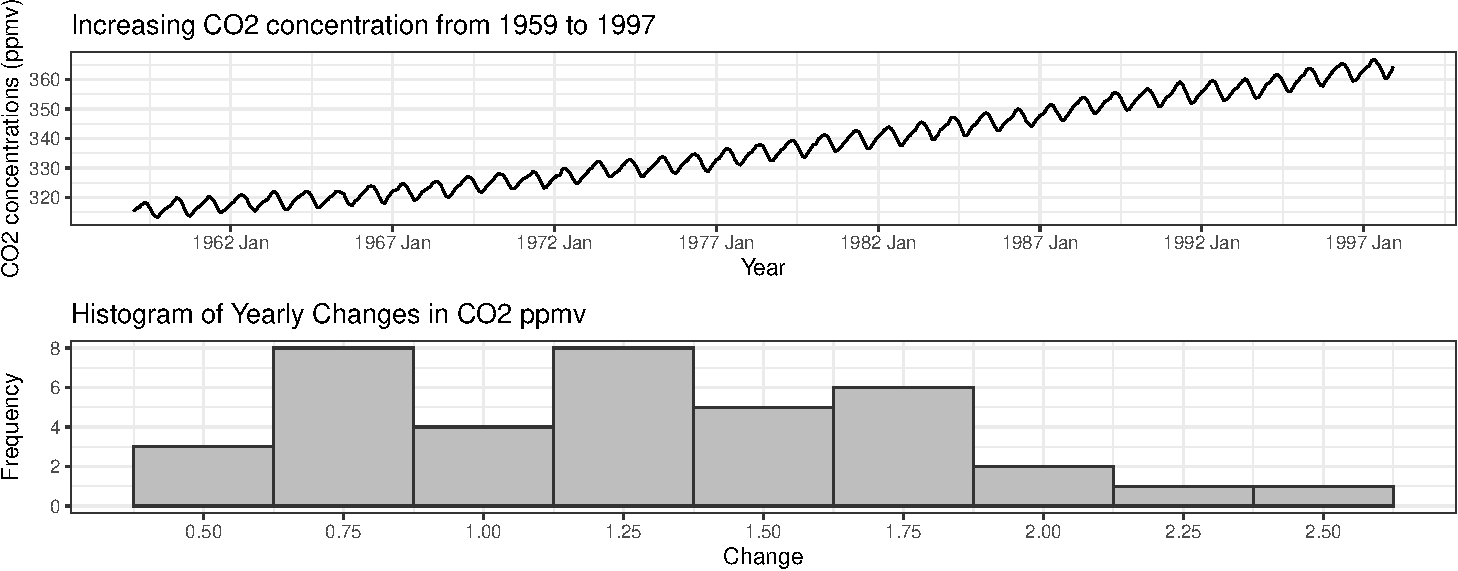
\includegraphics[width=1\linewidth]{lab_prompt_Updated_files/figure-latex/time-series-and-hist-1} 

}

\caption{Data source: CO2 measurements from Mauna Loa Observatory}\label{fig:time-series-and-hist}
\end{figure}

The time series also shows strong evidence of seasonality corresponding closely with the meteorological seasons of Autumn, Winter, Spring, and Summer. We now look at the ACF plot and average CO2 concentration for each month to gain further clarity on the seasonality.

\begin{figure}

{\centering 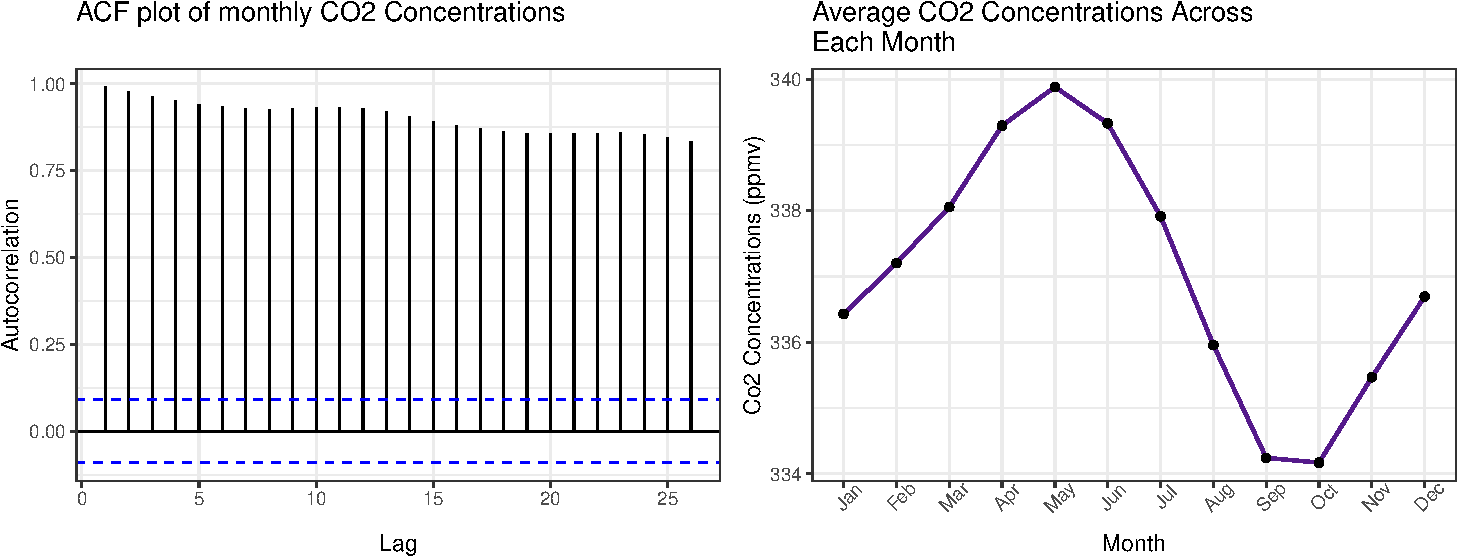
\includegraphics[width=1\linewidth]{lab_prompt_Updated_files/figure-latex/seasonality-eda-1} 

}

\caption{Observing seasonality in CO2 concentration}\label{fig:seasonality-eda}
\end{figure}

We also see a scallop/wave shaped pattern among correlations between the current value with growing lags. Clearer evidence of seasonality is shown when inspecting the monthly average the Co2 ppmv, when averaged across all years in the available data. CO2 contration peaks at the start of summer, and drops to a low in the fall, before rising again. This is likely due to the organic decomposition of plant life in these seasons (Keeling, 1960).

We now study the time series' stationarity. We first conduct the Augmented Dickey-Fuller Test to test the null hypothesis that the time series is not stationary. As seen in the time series plot for \texttt{co2}, we have a clear upward trend, suggesting non-stationarity. This is confirmed by a p-value of 0.2269 yielded by the test, which indicates insufficient evidence to reject the null hypothesis of non-stationarity. To look at stationarity in variance, we fit a yearly CO2 average on the monthly time series, and inspect the residuals from year to year. Although there are slight changes in the variance, they seem to regress to a constant variance over time. Thus, once we account for the yearly increases in CO2 ppmv, there is likely a constant variance over time.

\begin{figure}

{\centering 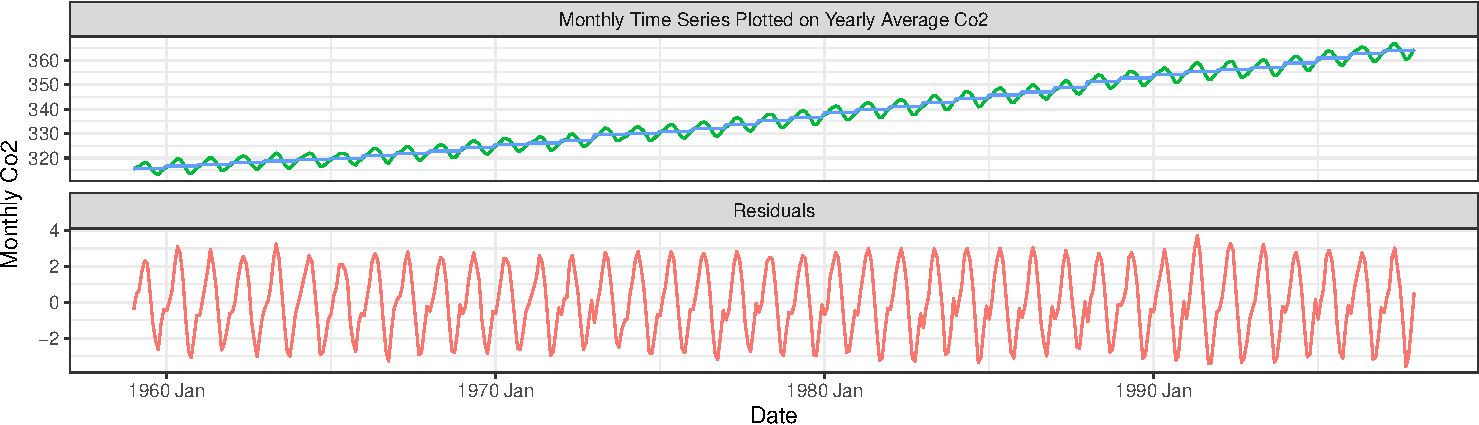
\includegraphics[width=1\linewidth]{lab_prompt_Updated_files/figure-latex/seasonality-irregularities-1} 

}

\caption{Studying variance over time}\label{fig:seasonality-irregularities}
\end{figure}

\newpage

\subsection{(3 points) Task 2a: Linear time trend model}\label{points-task-2a-linear-time-trend-model}

We now fit a linear time trend model the \texttt{co2} series, and examine the characteristics of the fit and residuals.

\begin{figure}

{\centering 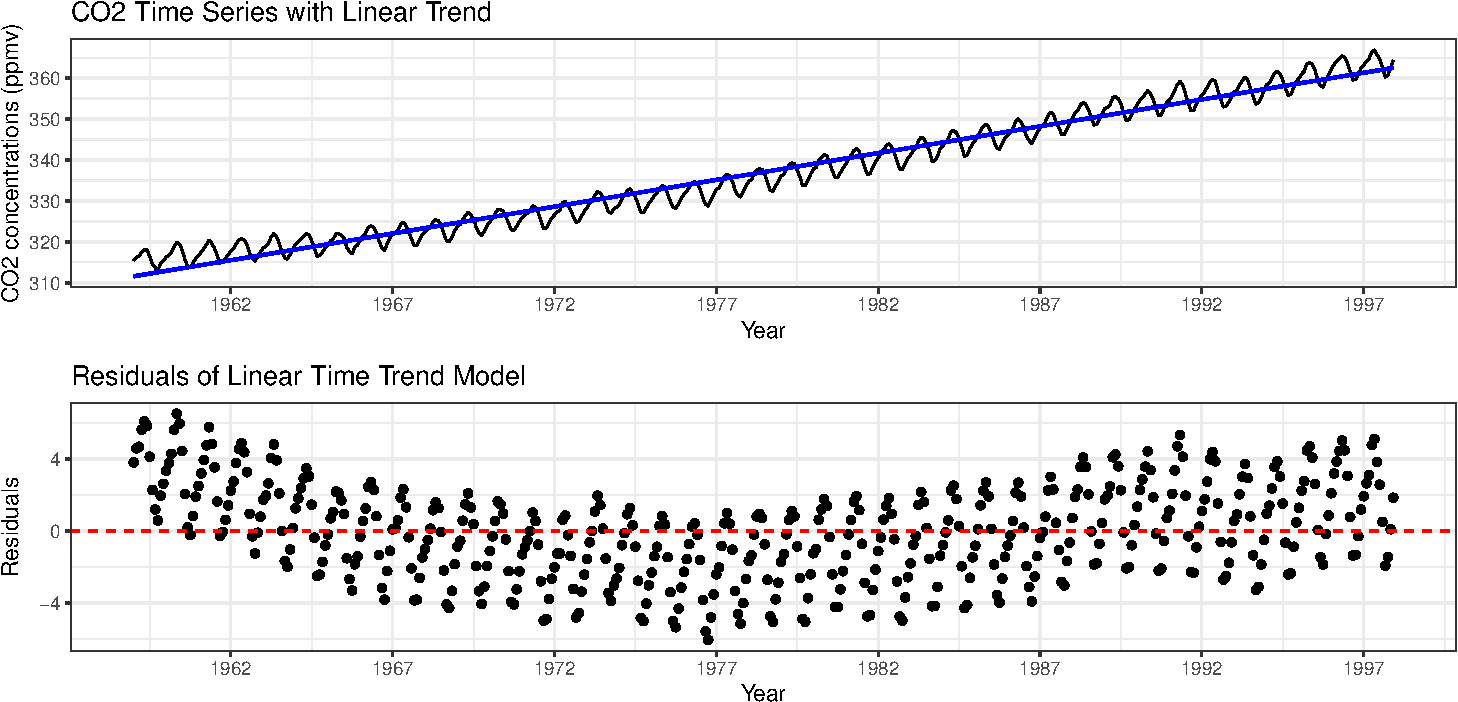
\includegraphics[width=1\linewidth]{lab_prompt_Updated_files/figure-latex/linear-model-plots-1} 

}

\caption{Evaluating a Linear Model}\label{fig:linear-model-plots}
\end{figure}

Upon inspection of linear fit, the fitted line appears to be systematically overestimating values at certain points and underestimating values at other points. This indicates that perhaps a higher order polynomial might produce a better fit of the overall trend. The residuals of the linear model also exhibit a cyclical, non-linear pattern, indicating that the model does not capture the seasonality in the data. The overall curve also suggests that the linear model insufficiently captures the overall trend. We now try a quadratic model, which may better capture the underlying trend.

\begin{figure}

{\centering 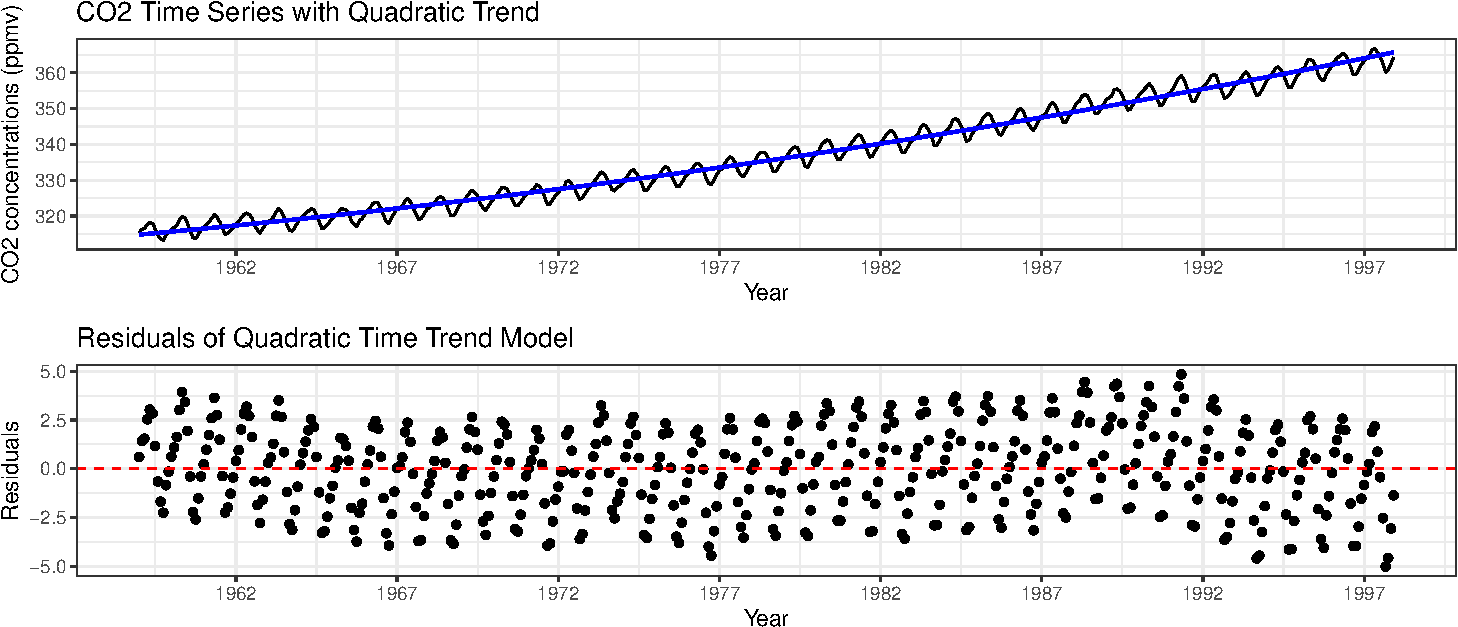
\includegraphics[width=1\linewidth]{lab_prompt_Updated_files/figure-latex/quadratic-model-plots-1} 

}

\caption{Evaluating a Quadratic Model}\label{fig:quadratic-model-plots}
\end{figure}

\newpage

The quadratic model's residuals indicate a small reduction in variance, demonstrating a slightly improved fit. However, the cyclical behavior remains, indicating that seasonality is unaccounted for in the model still. There is also an overall non-random trend in the residuals, indicating that the model still may not capture all the structural details. We now fit a polynomial model to the data to see if there is an improved fit.

\begin{figure}

{\centering 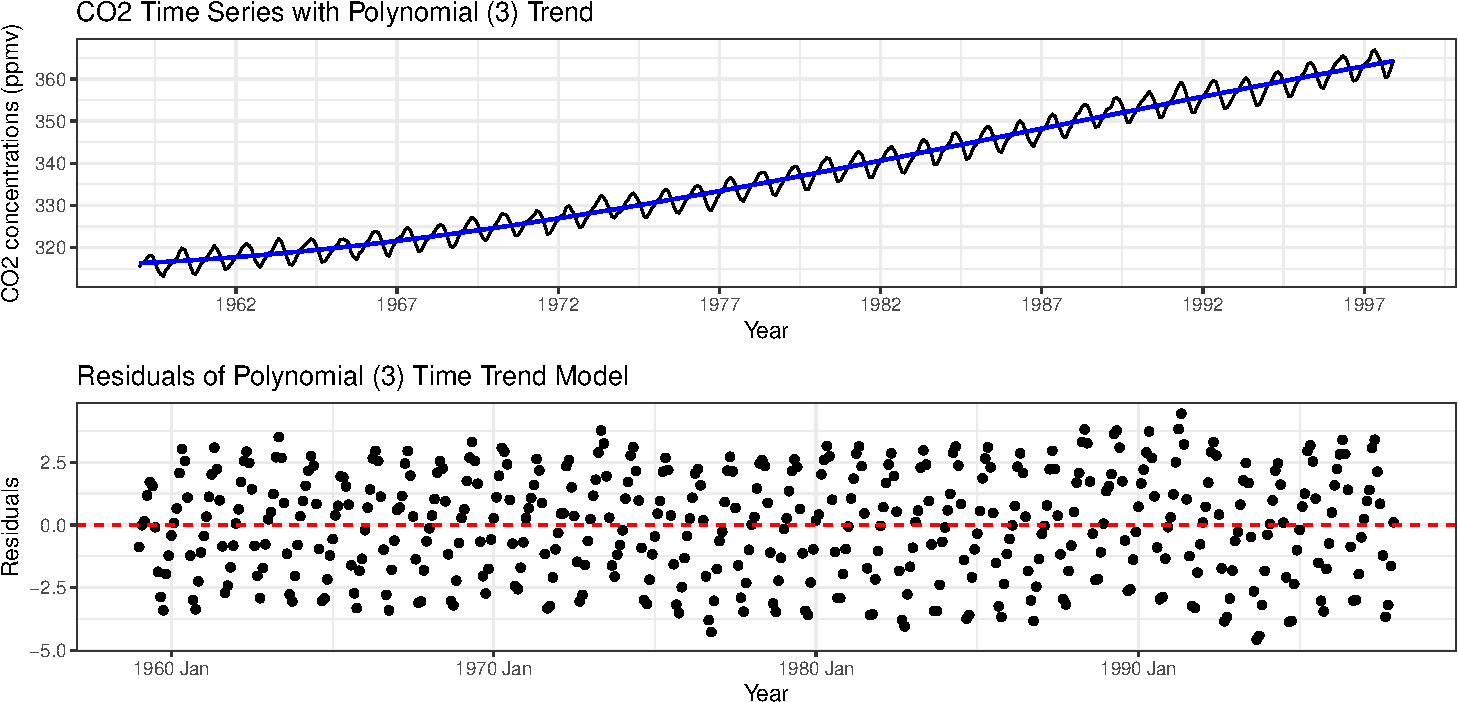
\includegraphics[width=1\linewidth]{lab_prompt_Updated_files/figure-latex/polynomial-model-plots-1} 

}

\caption{Evaluating a Polynomial (3) Model}\label{fig:polynomial-model-plots}
\end{figure}

The third-order polynomial model demonstrates improved residual behavior compared to quadratic and linear models. We chose to stop at this order to prevent excessive overfitting, as higher-order polynomials showed diminishing returns in model performance.

Apart from transforming the orders of the model, we were interested in data transformations - specifically logarithmic. As such we expermiented with a logarithmic dataset to observe the pattern of the data values.

\begin{figure}

{\centering 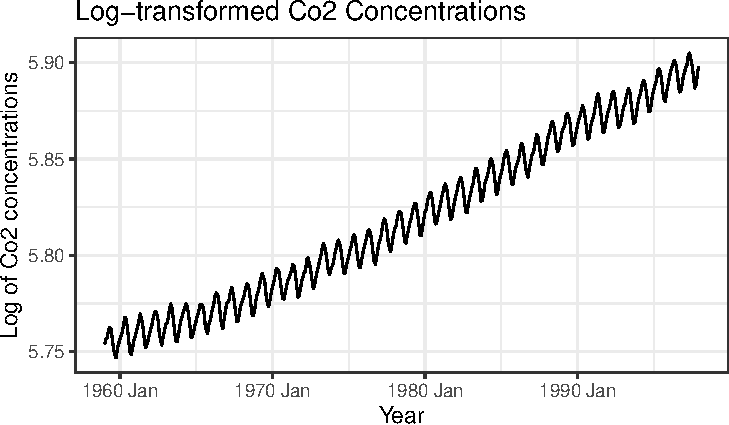
\includegraphics[width=0.8\linewidth]{lab_prompt_Updated_files/figure-latex/log-transformed-plot-1} 

}

\caption{Evaluating effect of taking a log on the series}\label{fig:log-transformed-plot}
\end{figure}

The logarithmic transformation reduces variance but offers minimal improvement compared to traditional plotting. This limited impact is likely due to the cyclical nature of the time series, which the transformation does not adequately address.

To address the cyclical behavior, we developed another polynomial model that includes each month as a variable. The average monthly CO2 emissions indicate significant cyclic patterns at the monthly level. By incorporating this variable, we anticipate an improvement in the fit of our time series model.

\begin{figure}

{\centering 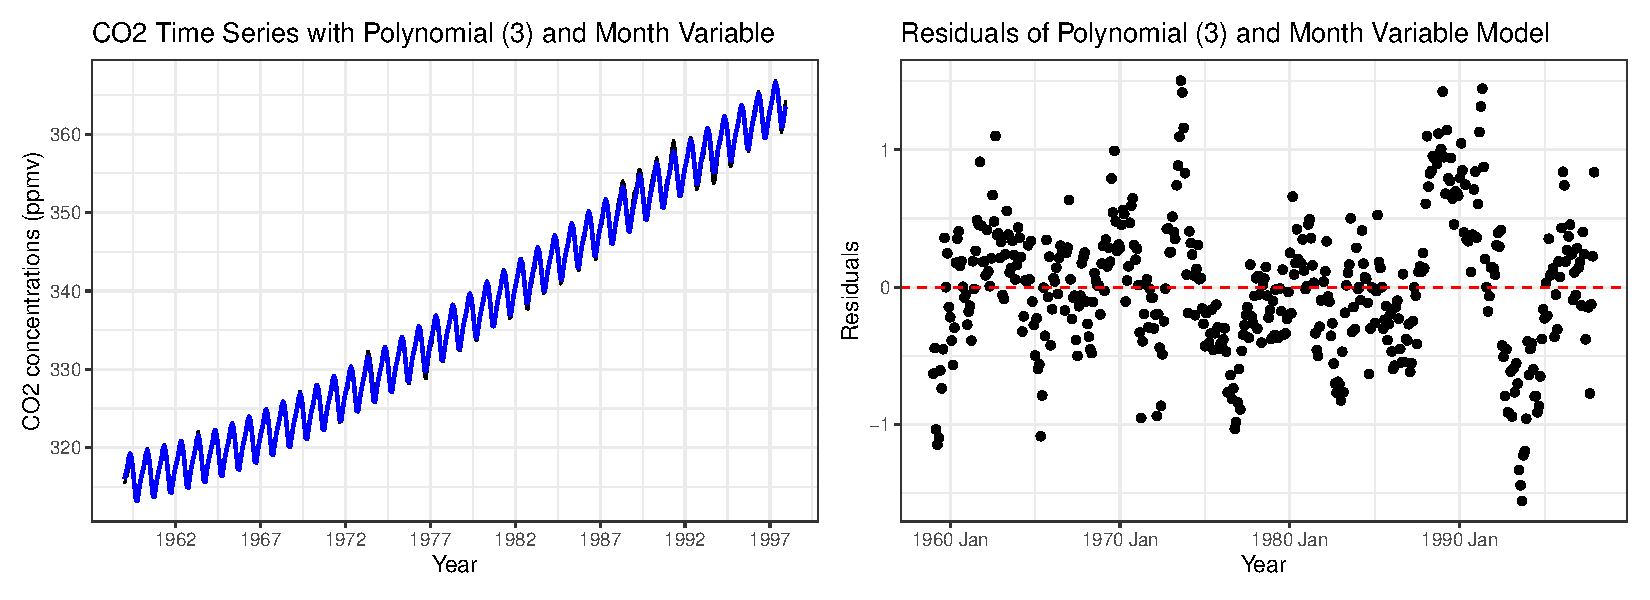
\includegraphics[width=1\linewidth]{lab_prompt_Updated_files/figure-latex/plot-month-1} 

}

\caption{Evaluating a Polynomial (3) with month variable model}\label{fig:plot-month}
\end{figure}

Incorporating the \texttt{month} dummy variable brought the residuals closer to zero, ranging between 1 and -1, but they still displayed a seasonal pattern. To refine the model, we grouped the months into quarters, to represent the seasons as a categorical variable, \texttt{season}.

\begin{figure}

{\centering 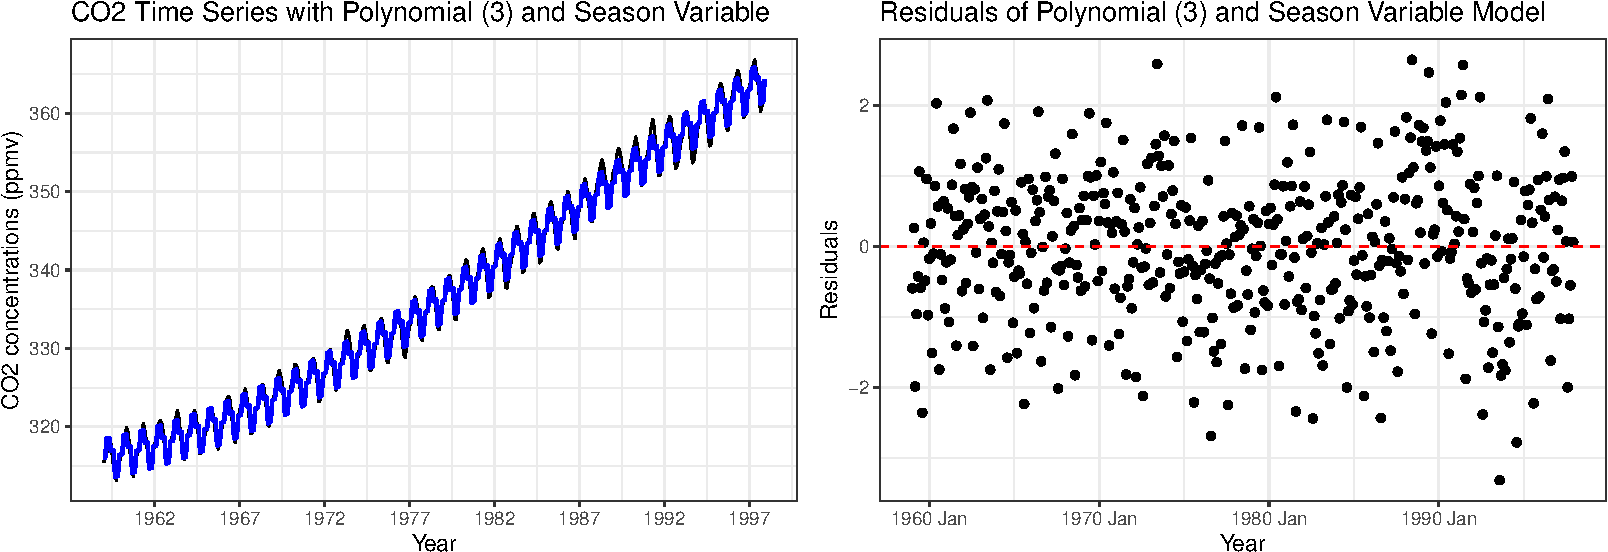
\includegraphics[width=1\linewidth]{lab_prompt_Updated_files/figure-latex/plot-seasonal-1} 

}

\caption{Evaluating a Polynomial (3) with season variable model}\label{fig:plot-seasonal}
\end{figure}

We see that using the \texttt{season} variable centered the residuals around zero with a random distribution, though fluctuations remained between 2 and -2. We now proceed with this model, the polynomial model with the \texttt{season} dummy variable, as it has the residuals plot that most look like a random distribution around the red line centered on zero, and developed a forecast for CO2 emissions through 2020.

\begin{figure}

{\centering 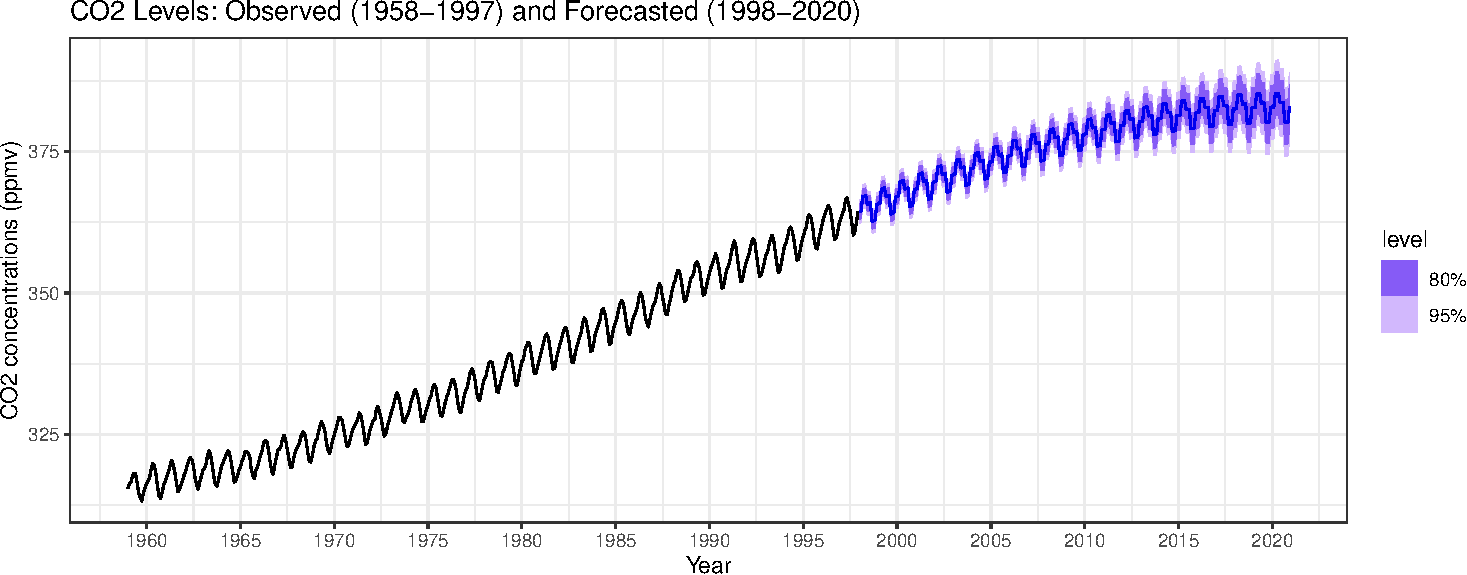
\includegraphics[width=1\linewidth]{lab_prompt_Updated_files/figure-latex/forecasting-model-1} 

}

\caption{Forecasting CO2 levels up to 2020 using a Polynomial (3) with month variable model}\label{fig:forecasting-model}
\end{figure}

The forecast model using the \texttt{season} variable shows decent performance, and predicts for the upward trend to persist up to 2020, along with the annual seasonality. We will now explore an ARIMA model to see if it may better capture the time series' underlying patterns and improve forecast accuracy.

\subsection{(3 points) Task 3a: ARIMA times series model}\label{points-task-3a-arima-times-series-model}

As seen in our EDA, there is non-stationarity. Thus, we will proceed to difference the data to make it stationary, both at the 1st lag followed by the 12th lag to account for seasonality, which is a crucial step before fitting the ARIMA model effectively.

\begin{figure}

{\centering 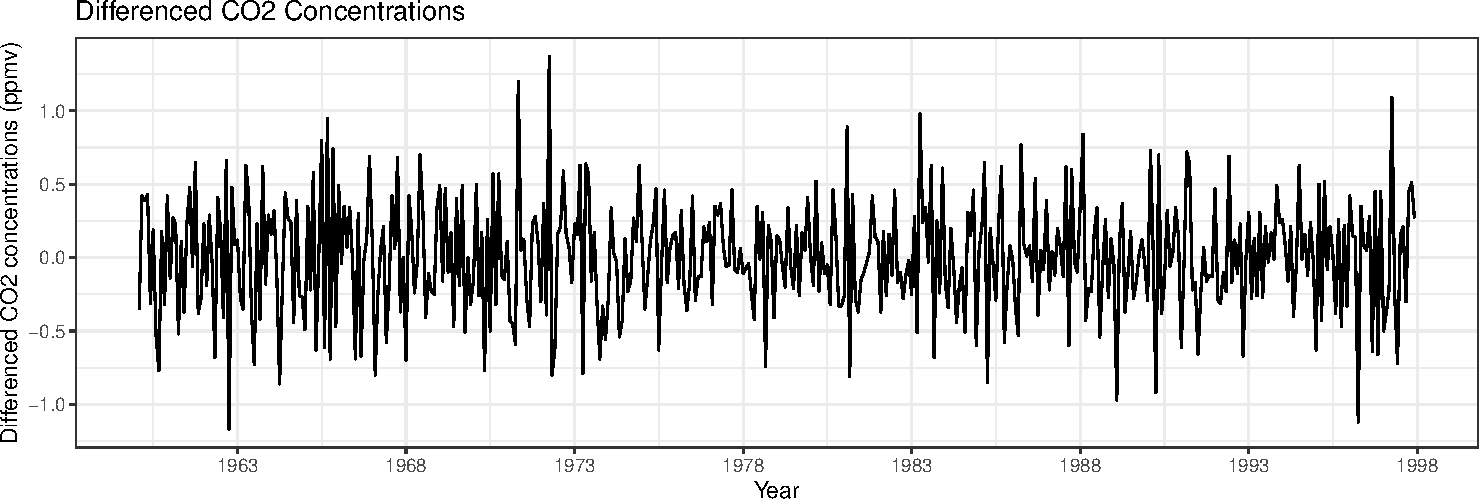
\includegraphics[width=1\linewidth]{lab_prompt_Updated_files/figure-latex/arima-differencing-1} 

}

\caption{Differenced series looks more stationary in the mean and variance}\label{fig:arima-differencing}
\end{figure}

The plot of the differenced time series does look more stationary in the mean and variance; which is confirmed by a 0.01 p-value yielded from the Augmented Dickey-Fuller Test, indicating sufficient evidence to reject the null hypothesis of non-stationarity. We now look at the ACF and PACF plots of the differenced time series, to inform how we should construct our ARIMA model.

\newpage

\begin{figure}

{\centering 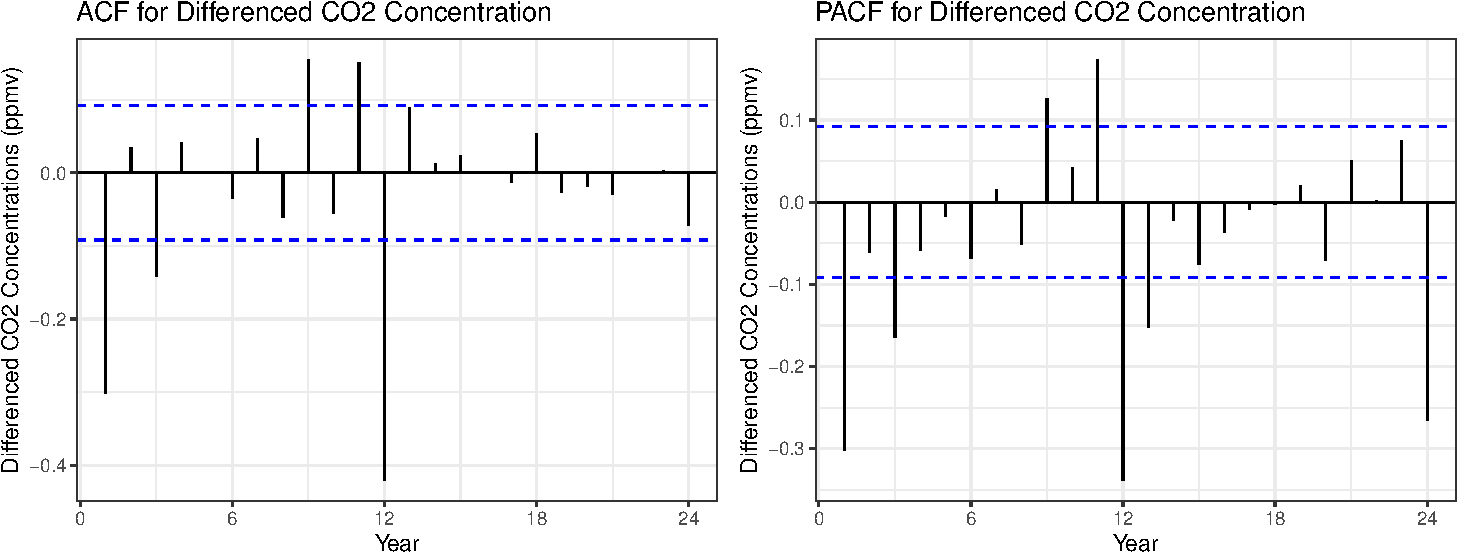
\includegraphics[width=1\linewidth]{lab_prompt_Updated_files/figure-latex/acf-pacf-1} 

}

\caption{Evaluating ACF and PACF for differenced series}\label{fig:acf-pacf}
\end{figure}

Both ACF and PACF plots show strong auto-correlation with lag 1, and the ACF cutting off strong after lag 1, and the PACF having a significant spike at lag 1, and tapering off a little more. This might indicate that our model has a MA(1) component. The spike at lag 12 in the ACF might also indicate a seasonal MA component.

The ARIMA function behaved as expected, and returned an ARIMA(0,1,1)(0,1,1)\(_{12}\) function, with BIC = 182.32. We will now look at the residuals for this model.

\begin{figure}

{\centering 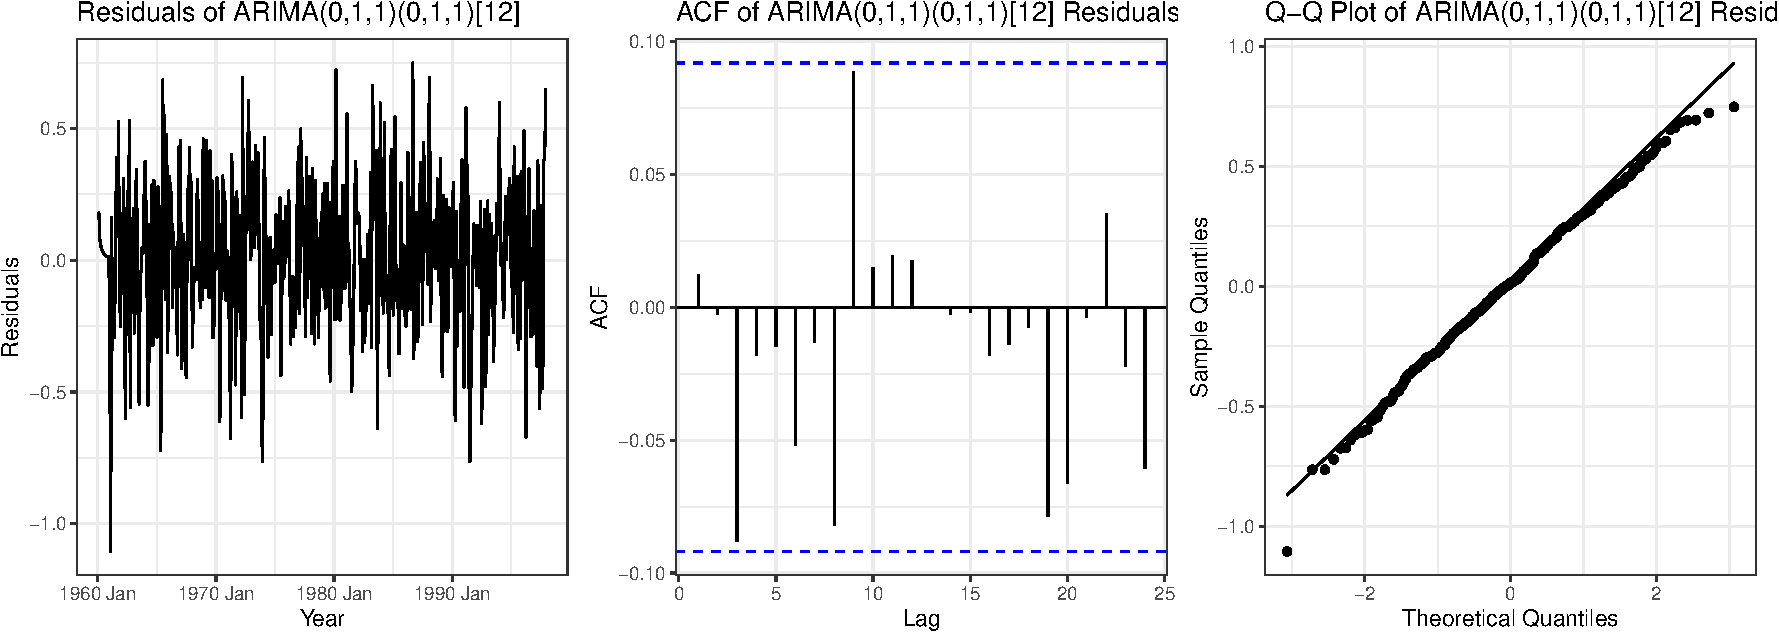
\includegraphics[width=1\linewidth]{lab_prompt_Updated_files/figure-latex/arima-residuals-1} 

}

\caption{Evaluating ARIMA model }\label{fig:arima-residuals}
\end{figure}

The residuals look random, there are no significant autocorrelations in the ACF, and they closely follow a a normal distribution in the Q-Q plot. These all indicate that the model has captured most of the underlying structure of our time series. A Ljung-Box test also yielded a p-value of 0.6733, further confirming that there is insufficient statistical evidence to reject the null hypothesis that there is no autocorrelation. We can proceed with forecasting the time series data through 2022.
\newpage

\begin{figure}[H]

{\centering 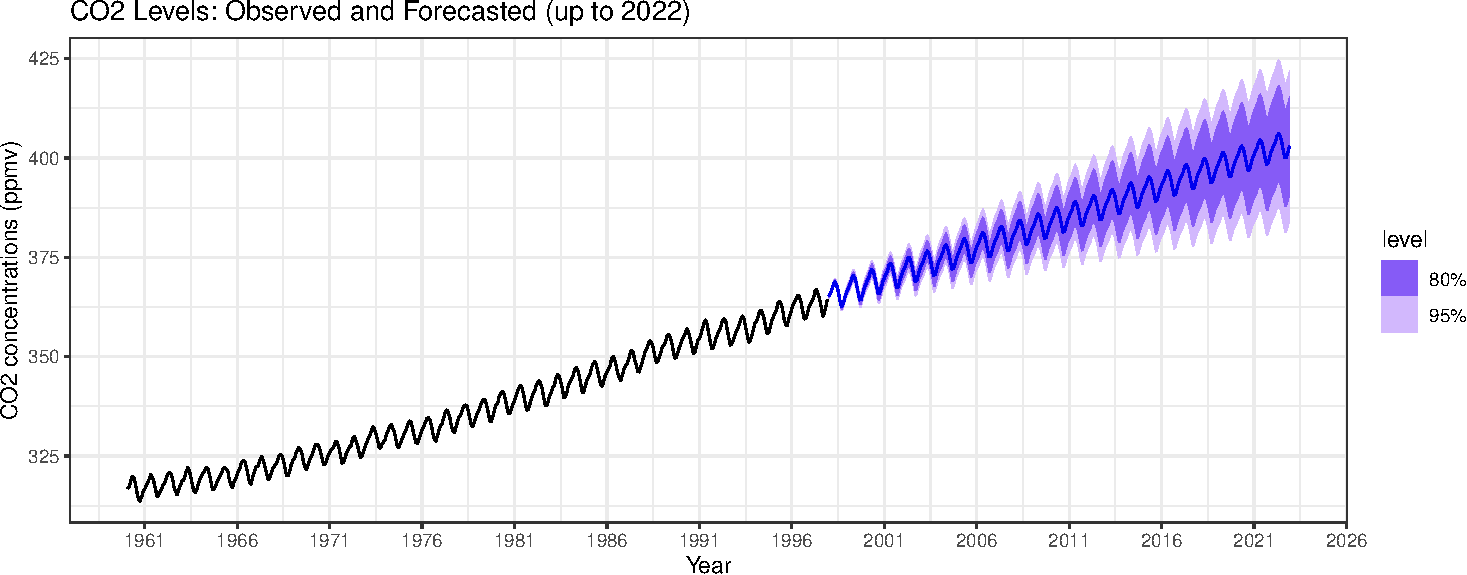
\includegraphics[width=1\linewidth]{lab_prompt_Updated_files/figure-latex/arima-forecasting-1} 

}

\caption{Forecasting up to 2022 using an ARIMA model}\label{fig:arima-forecasting}
\end{figure}

\subsection{(3 points) Task 4a: Forecast atmospheric CO2 growth}\label{points-task-4a-forecast-atmospheric-co2-growth}

We now forecast when atmospheric CO2 is expected to be at 420 ppm and 500 ppm for the first and final times, as seen in the table below.

\textbackslash begin\{table\}{[}H{]}
\centering
\textbackslash caption\{\label{tab:forecastone}CO2 Levels and Forecasted Times with 80\% Confidence Intervals\}
\centering
\fontsize{9}{11}\selectfont

\begin{tabular}[t]{l|l|l|l|l}
\hline
CO2.Level & First.Month & First.Value & Last.Month & Last.Value\\
\hline
420 ppm & 2031 May & 420.1 (402.3, 438.0) & 2035 Oct & 420.4 (399.5, 441.3)\\
\hline
500 ppm & 2083 Apr & 500.4 (437.9,562.9) & 2085 Dec & 500.9 (435.7,566.2)\\
\hline
\end{tabular}

\textbackslash end\{table\}

Our model also forecasts CO2 levels in the year 2100. Although these forecasts include a standard deviation, but these do not take into account the existing efforts to reduce global greenhouse gases, such as \textbf{insert efforts here}. Thus, since these are very human-activty dependent, it is unlikely to be super accurate.

\begin{table}[H]
\centering
\caption{\label{tab:forecasttwo}CO2 Forecasts in 2100}
\centering
\fontsize{9}{11}\selectfont
\begin{tabular}[t]{l|r|r}
\hline
Date & Value & SD\\
\hline
2100 Jan & 523.7 & 62.8\\
\hline
2100 Feb & 524.6 & 62.9\\
\hline
2100 Mar & 525.5 & 63.0\\
\hline
2100 Apr & 526.8 & 63.0\\
\hline
2100 May & 527.4 & 63.1\\
\hline
2100 Jun & 526.7 & 63.2\\
\hline
2100 Jul & 525.2 & 63.3\\
\hline
2100 Aug & 523.1 & 63.3\\
\hline
2100 Sep & 521.3 & 63.4\\
\hline
2100 Oct & 521.4 & 63.5\\
\hline
2100 Nov & 522.8 & 63.5\\
\hline
2100 Dec & 524.2 & 63.6\\
\hline
\end{tabular}
\end{table}

\newpage

\section{Report from the Point of View of the Present}\label{report-from-the-point-of-view-of-the-present}

\subsection{(1 point) Task 0b: Introduction}\label{point-task-0b-introduction}

Following our initial evaluation using Keeling's data, we now seek to re-examine the original study to identify potential deviations in CO2 level predictions. Specifically, we aim to discern whether any discrepancies between predicted and actual CO2 levels since 1997 arise from the inherent limitations of prior models or from changes within the CO2-generating system itself.

Before 1997, CO2 data was collected using a chemical gas analyzer that relied on infrared absorption to measure monthly CO2 concentrations from January 1959 through December 1997. The present data collection approach, however, leverages a newer CO2 analyzer installed at Mauna Loa, employing Cavity Ring-Down Spectroscopy (CRDS). CRDS determines CO2 concentration by measuring the rate at which light is absorbed in an optical cavity, rather than the intensity. This method offers significant advantages, as it eliminates dependencies on light intensity and sample path length, providing absolute, highly accurate concentration measurements without frequent recalibration. Furthermore, CRDS is capable of hourly measurements, and its rigorous gas-flushing system ensures each sample's reliability. These improvements in measurement precision and frequency offer researchers enhanced insight into CO2 trends, facilitating a more robust evaluation of the models' predictive capabilities and any potential systemic changes.

\subsection{(3 points) Task 1b: Create a modern data pipeline for Mona Loa CO2 data.}\label{points-task-1b-create-a-modern-data-pipeline-for-mona-loa-co2-data.}

We created a data pipeline, pulling the most recent weekly data from the \href{https://gml.noaa.gov/ccgg/trends/data.html}{Global Monitoring Laboratory} page. We now conduct a similar EDA for the updated time series data from Dr.~Xin Lan's study of CO2 atmospheric trends.

We first plot the time series data for CO2 concentrations, and a histogram of the yearly changes.

\begin{figure}

{\centering 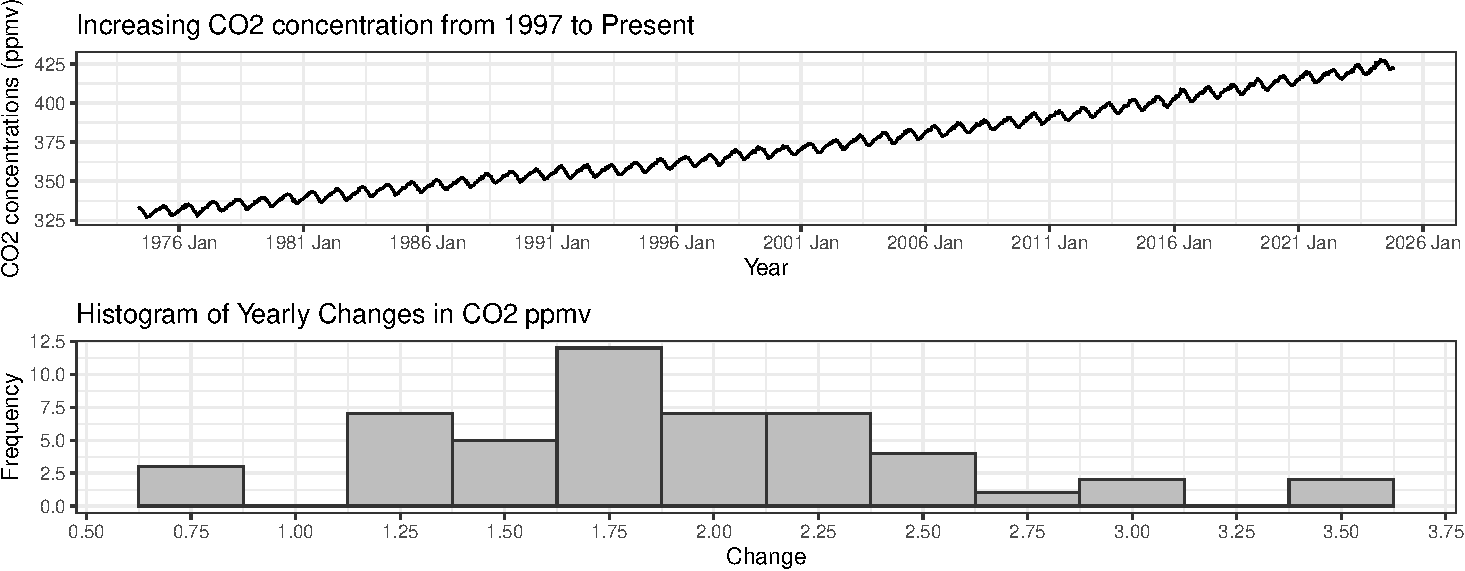
\includegraphics[width=1\linewidth]{lab_prompt_Updated_files/figure-latex/time-series-and-hist-two-1} 

}

\caption{Data source: CO2 measurements from Mauna Loa Observatory}\label{fig:time-series-and-hist-two}
\end{figure}

From 1998 to 2024, the time series continues to show a clear upward trend of global CO2 concentrations, with an average increase in 1.90 CO2 ppmv and a standard deviation of .61 CO2 ppmv. These are larger values than those calculated in 1997, indicating that the time series had a larger average increase and standard deviation from 1998 to present day 2024. The histogram also shows a rightward shift in the distribution, indicating that the annual changes have increased.

We now look at the ACF plot and weekly CO2 concentration across every year to gain further clarity on the seasonality.
\newpage

\begin{figure}

{\centering 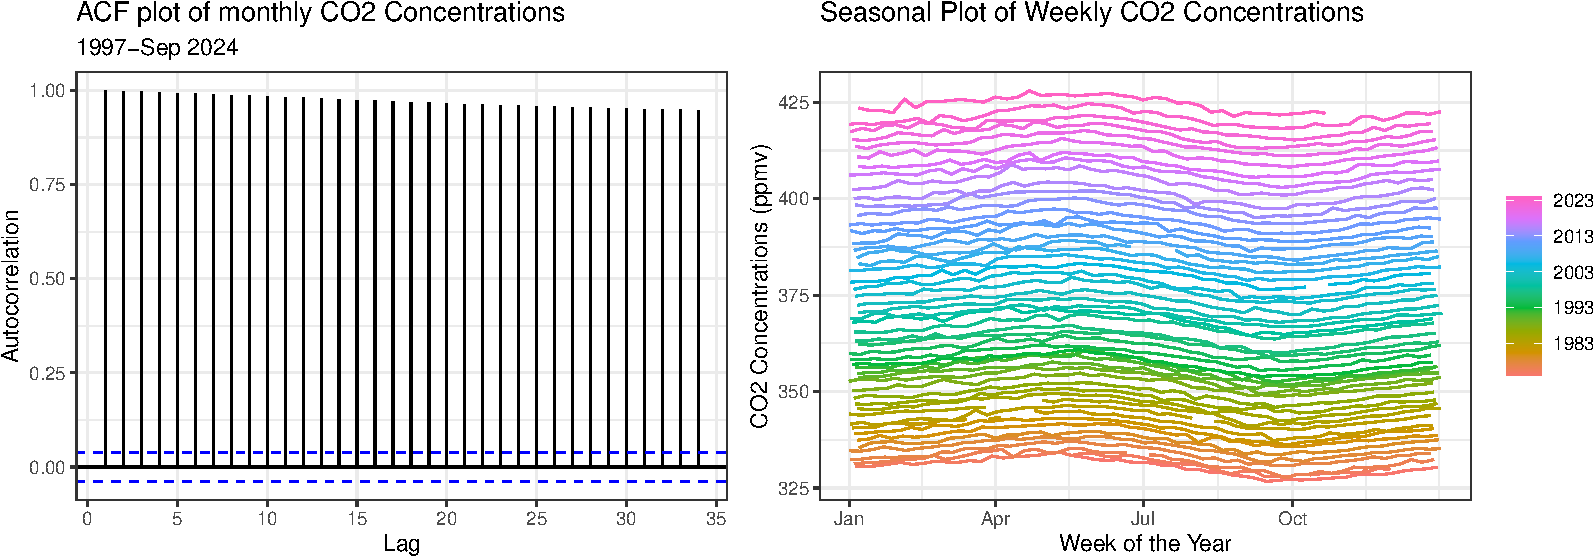
\includegraphics[width=1\linewidth]{lab_prompt_Updated_files/figure-latex/seasonality-eda-two-1} 

}

\caption{Observing seasonality in CO2 concentration}\label{fig:seasonality-eda-two}
\end{figure}

We see strong persistent autocorrelation for many lags, indicating an overall trend. The time series also shows strong evidence of seasonality corresponding closely with the meteorological seasons: CO2 concentration peaks at the start of summer, and drops to a low in the fall, before rising again. These observations are consistent with the report from 1997.

We now study the time series' stationarity. We conduct the Augmented Dickey-Fuller Test to test the null hypothesis that the time series is not stationary. As seen in the time series plot for \texttt{co2}, we have a clear upward trend, suggesting non-stationarity. However, this is \emph{contrasted} by a p-value of 0.01 yielded by the test, which indicates evidence to reject the null hypothesis of non-stationarity. To look at stationarity in variance, we fit a yearly CO2 average on the monthly time series, and inspect the residuals from year to year. Although there are slight changes in the variance, they seem to regress to a constant variance over time. Thus, once we account for the yearly increases in CO2 ppmv, there is likely a constant variance over time.

\begin{figure}

{\centering 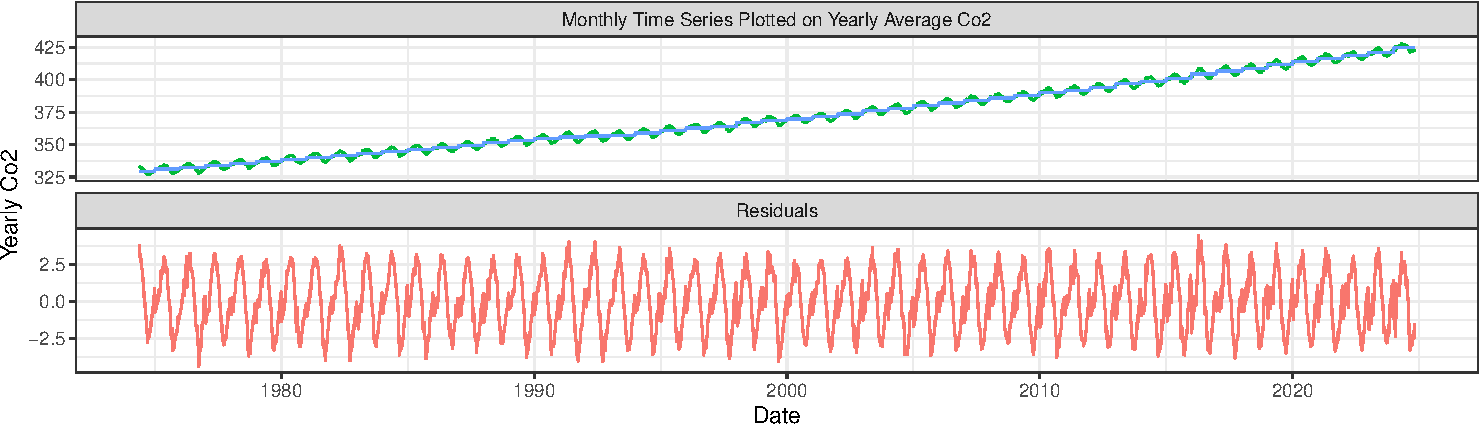
\includegraphics[width=1\linewidth]{lab_prompt_Updated_files/figure-latex/seasonality-irregularities-two-1} 

}

\caption{Studying variance over time}\label{fig:seasonality-irregularities-two}
\end{figure}

The new data collection method and techniques yield similar trends in average CO2 levels across months and years, with no notable deviations from prior patterns. Additionally, the residuals display consistent patterns, indicating that the updated methods align closely with previous data quality and trend behavior. The only detected change was the results of the adf test which found the CO2 values to be stationary.

\newpage

\subsection{(1 point) Task 2b: Compare linear model forecasts against realized CO2}\label{point-task-2b-compare-linear-model-forecasts-against-realized-co2}

\begin{figure}

{\centering 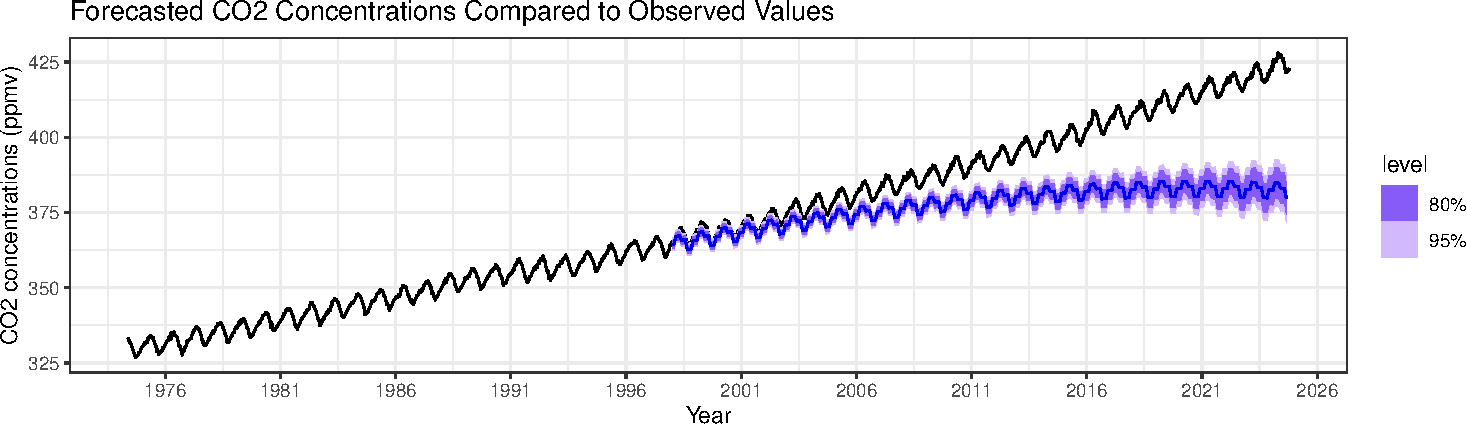
\includegraphics[width=1\linewidth]{lab_prompt_Updated_files/figure-latex/comparing-to-forecast-1} 

}

\caption{Forecasted with a Polynomial (3) with Season Variable Model}\label{fig:comparing-to-forecast}
\end{figure}

When plotting the observed Co2 concentrations to the forecasted values from data up to 1997, we see a clear mismatch in predictions. The model had predicted a declining trend of Co2 concentrations, but actual concentrations increased fairly linearly. The declining trend was modeled with an expected curvilinear relationship with Co2 concentrations over time, as this fit better when looking at the time period between the 1950s and 1990s. But the actual time series may not be appropriately measured as a strict polynomial relationship, possibly depending on external causes such as human-lead efforts to reduce carbon emissions or efforts to restrict policy against reducing carbon emissions.

\subsection{(1 point) Task 3b: Compare ARIMA models forecasts against realized CO2}\label{point-task-3b-compare-arima-models-forecasts-against-realized-co2}

\begin{figure}

{\centering 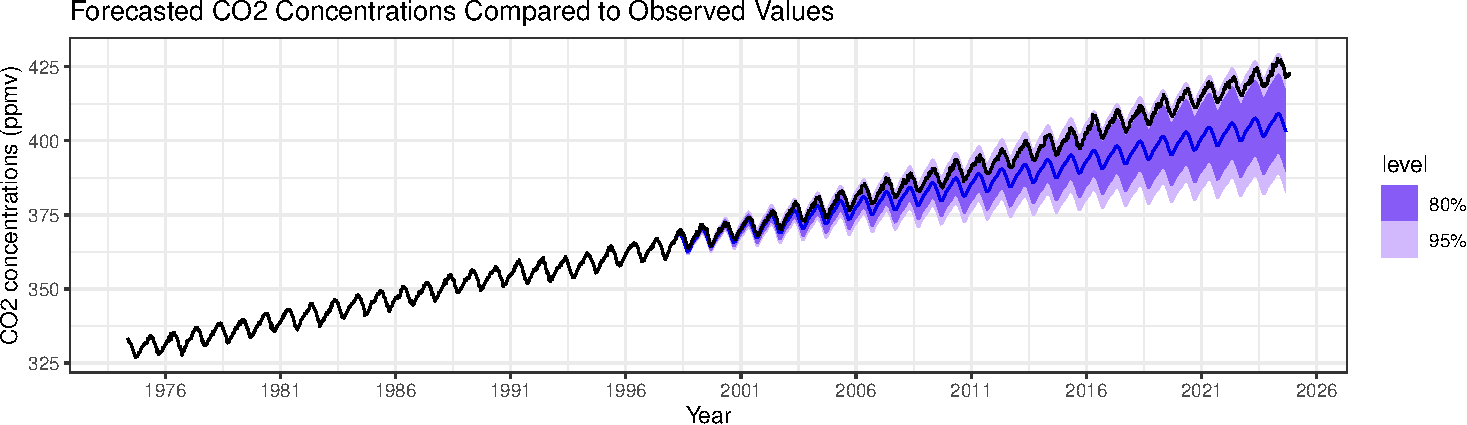
\includegraphics[width=1\linewidth]{lab_prompt_Updated_files/figure-latex/comparing-to-arima-1} 

}

\caption{Forecasted with a ARIMA Model}\label{fig:comparing-to-arima}
\end{figure}

The ARIMA model, while closer in trend to the observed values than the curvilinear model, still underestimates the increases in global Co2 concentrations. The yearly fluctuations match better than the previous forecast and in the short-term the forecast performs well, but within 5 years the forecast diverges from actual concentrations and by 2020 we see concentrations of \textasciitilde12.5 Co2 ppmv higher than anticipated. By 2024, the observed values at barely at the tail end of the 95\% confidence interval, and look unlikely to stay within the confidence interval should the forecast continue.

\subsection{(3 points) Task 4b: Evaluate the performance of 1997 linear and ARIMA models}\label{points-task-4b-evaluate-the-performance-of-1997-linear-and-arima-models}

Before, we expected that we would reach 420 ppmv around May of 2031, but the first date we past this threshold was in March of 2022. In other words, our predictions were nearly a decade off courses. This may imply a more concerning trajectory for negative environmental outcomes than previously anticipated.

We now use the weekly data to generate a month-average series from 1997 to present-day 2024, and compare the overall forecasting performance of both the Polynomial (3) with Season variable model, and the ARIMA model.

We do this by first comparing the Mean Absolute Error (MAE) and Root Mean Squared Error (RMSE) of each forecasting model, and conduct a significance test to formally compare the differences. We see that the polynomial season model has an MAE of \textasciitilde{} 15.8, while the ARIMA model has lower MAE of \textasciitilde{} 7.3. Similarly, we see that the polynomial season model has a higher RMSE of \textasciitilde{} 19.9, while the ARIMA model has lower RMSE of \textasciitilde{} 8.9. That the ARIMA model has lower errors suggests that it is a better fitting forecasting model. Finally, the conducted Diebold-Mariano Test, which tests for differences in forecast errors, returns a significant p-value of less than 2.2e-16, allowing us to reject the null hypothesis that the two forecasts have the same forecast accuracy.

\subsection{(4 points) Task 5b: Train best models on present data}\label{points-task-5b-train-best-models-on-present-data}

We now seasonally adjust the weekly data, and split both seasonally-adjusted (SA) and non-seasonally-adjusted (NSA) series into training and test sets, using the last two years (2022-2024) of observations as the test sets. We also use spline interpolation for 18 missing values. We obtain the decomposition in the plots below.

\begin{figure}

{\centering 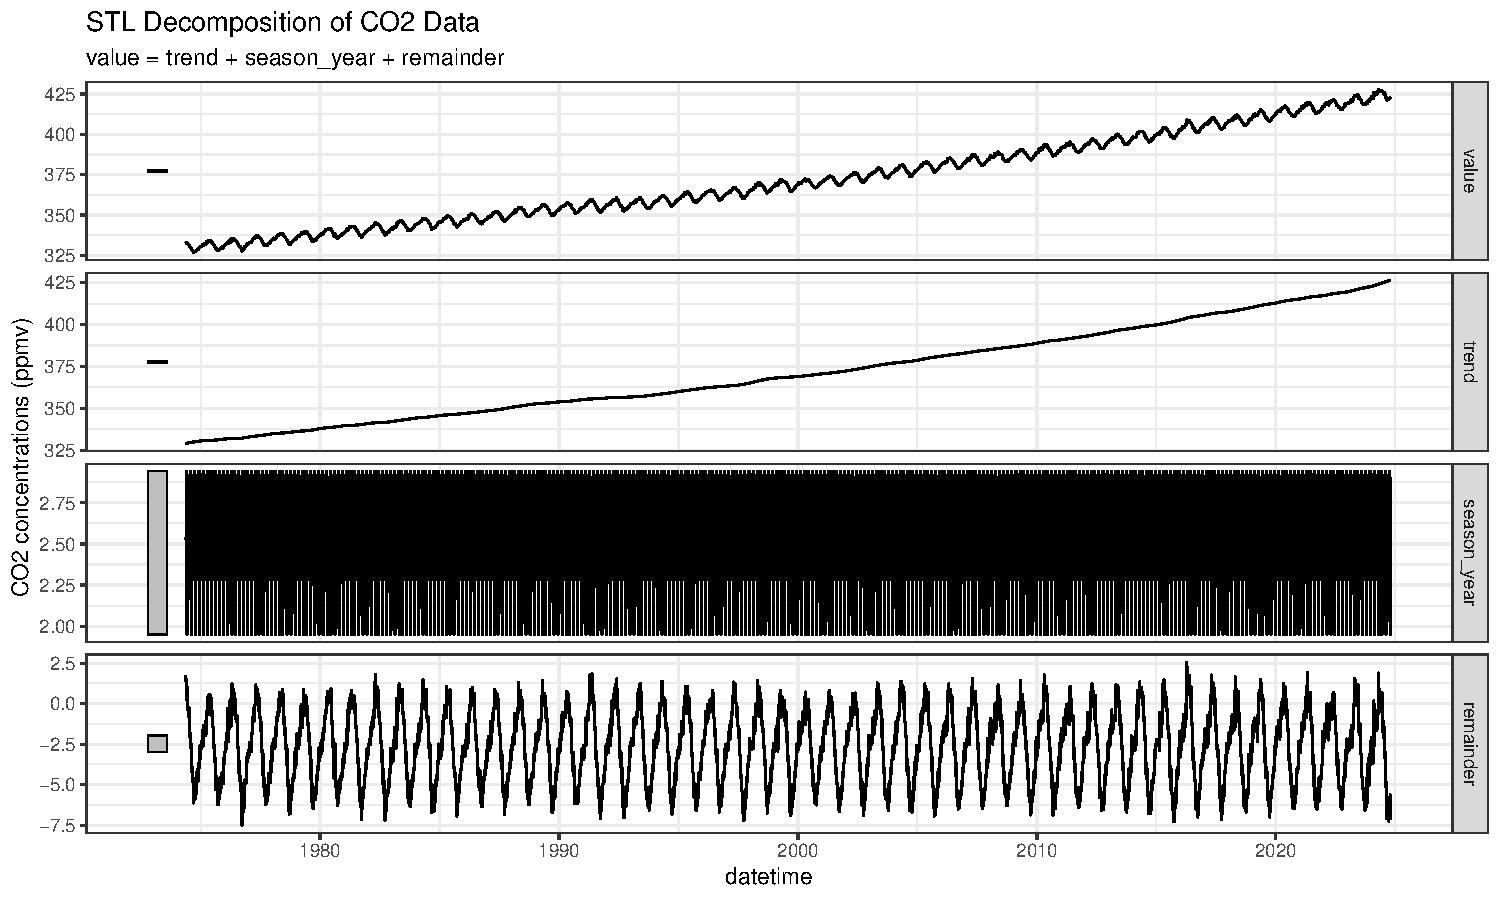
\includegraphics[width=1\linewidth]{lab_prompt_Updated_files/figure-latex/stl-decomposition-1} 

}

\caption{Clear seasonality and trend seen from decomposition}\label{fig:stl-decomposition}
\end{figure}

We now look at the ACFs and PACFs of the SA and NSA training data, with a difference of 1 to account of the overall trend, to consider what ARIMA models we can fit to it.

\newpage

\begin{figure}

{\centering 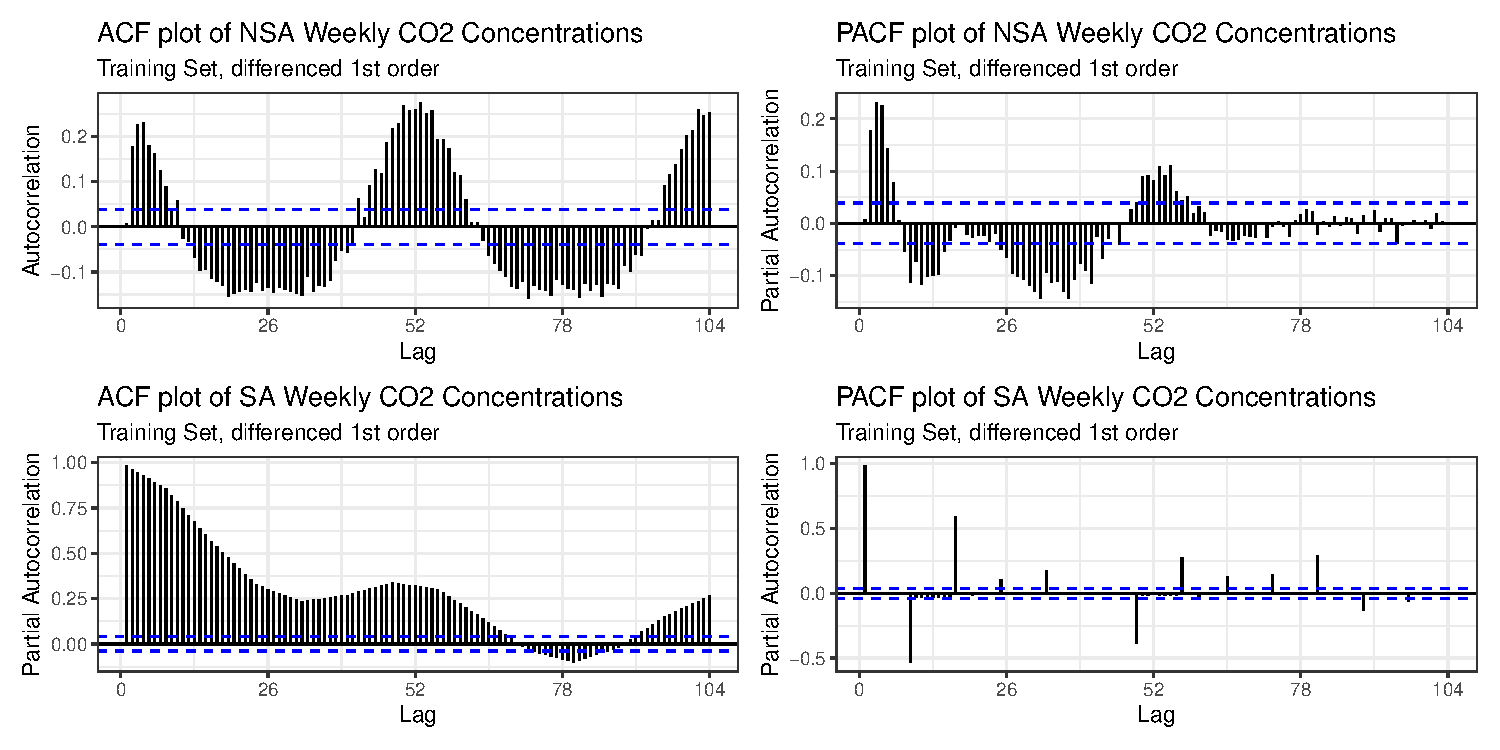
\includegraphics[width=1\linewidth]{lab_prompt_Updated_files/figure-latex/acf-and-pacfs-1} 

}

\caption{EDA on training and test sets}\label{fig:acf-and-pacfs}
\end{figure}

We note that the NSA ACF shows clear seasonality, indicating that should include a seasonal difference. The NSA PACF also shows significant autocorrelation up to the first 13 lags. Given that both ACFs and PACFs have some tapering off and show clear seasonality, we should try both an AR and MA model with a seasonal difference and seasonal AR and MA components, perhaps ARIMA(1,1,1)(1,1,1). We will also let the \texttt{ARIMA} function choose a model for us.

For the SA data, since it was already de-trended and we also see a tapering ACF and sharply dropping PACF, we will try a ARIMA(1,1,0), ARIMA(1,1,1), and ARIMA(2,1,0). We get the tables below.

\begin{table}[H]
\centering
\caption{\label{tab:nsa-table}NSA ARIMA Model Results}
\centering
\fontsize{9}{11}\selectfont
\begin{tabular}[t]{l|r|r|r}
\hline
Model & AICc & BIC & LogLik\\
\hline
ARIMA(1,1,1)(0,1,1) & 3045.33 & 3068.564 & -1518.657\\
\hline
Auto: ARIMA(0,1,3)(2,1,0) & 3332.50 & 3361.537 & -1661.238\\
\hline
\end{tabular}
\end{table}

\begin{table}[H]
\centering
\caption{\label{tab:sa-table}SA ARIMA Model Results}
\centering
\fontsize{9}{11}\selectfont
\begin{tabular}[t]{l|r|r|r}
\hline
Model & AICc & BIC & LogLik\\
\hline
ARIMA(1,1,0) & -22965.48 & -22947.99 & 11485.74\\
\hline
ARIMA(1,1,1) & -22963.67 & -22940.35 & 11485.84\\
\hline
ARIMA(2,1,0) & -22963.67 & -22940.35 & 11485.84\\
\hline
\end{tabular}
\end{table}

For the NSA data, we will pick the model that has the lowest IC values, ARIMA(1,1,1)(0,1,1), as it clearly outperforms the model picked by the \texttt{ARIMA} function.For SA data, all models are almost par; we will thus choose the parsimonious model of ARIMA(1,1,0). We now look at the forecasts of these two models on our test data. We now look at both the fit of our models on the actual data, as well as the forecasts for both models.

\newpage

\begin{figure}

{\centering 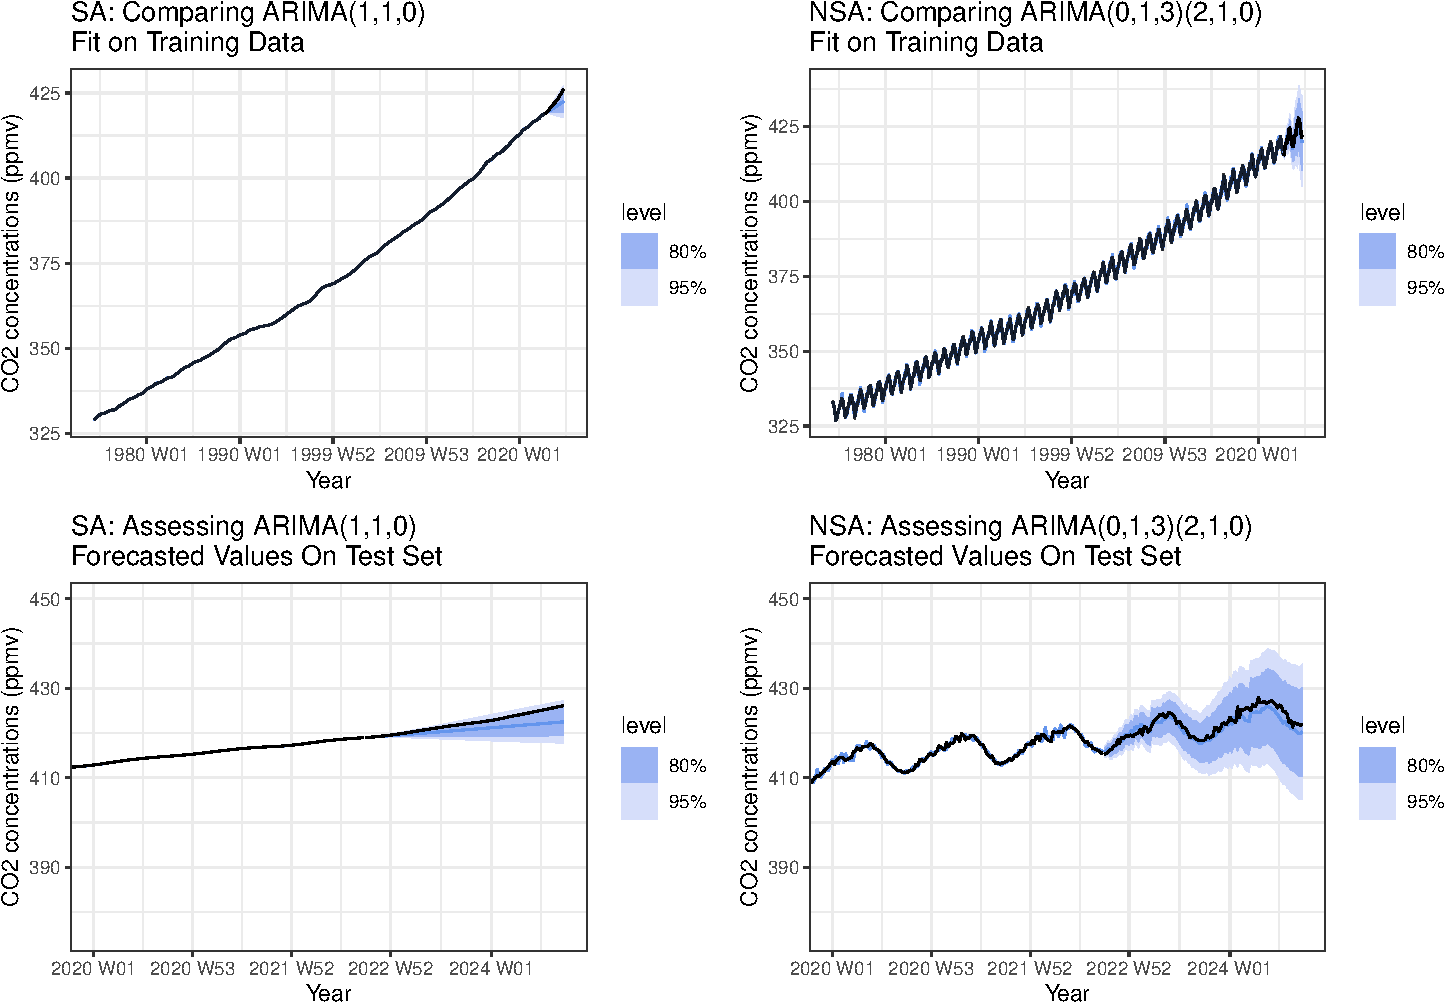
\includegraphics[width=1\linewidth]{lab_prompt_Updated_files/figure-latex/final-forecasts-1} 

}

\caption{Assessing ARIMA Models on NSA and SA data}\label{fig:final-forecasts}
\end{figure}

We can see that our models' fitted values in blue are extremely close to the actual values plotted in black in the top two plots. For the forecasts, both models 95\% confidence intervals in blue included the actual data in black However, the NSA model seemed to provide a closer fit to the actual data. We now compare both the RMSE and MAE of both models.

\begin{table}[H]
\centering
\caption{\label{tab:final-models-comparison-table}Comparison of NSA and SA Models on Training and Test Sets}
\centering
\fontsize{9}{11}\selectfont
\begin{tabular}[t]{l|r|r}
\hline
Metric & NSA.ARIMA.Model & SA.ARIMA.Model\\
\hline
RMSE (Training) & 0.4404618 & 0.0070277\\
\hline
MAE (Training) & 0.3347048 & 0.0009972\\
\hline
RMSE (Test) & 0.9844368 & 1.7873662\\
\hline
MAE (Test) & 0.8016645 & 1.4385201\\
\hline
\end{tabular}
\end{table}

As we see from the table above, the SA model outperformed the NSA model on the training set in both RMSE and MAE metrics, but the NSA model outperformed the SA model on the test set, indicating that the NSA model of ARIMA(1,1,1)(0,1,1) generalizes better. Given that our SA ARIMA model can be improved, we now fit a polynomial time-trend model for the SA series and compare it with the SA ARIMA model.

\newpage

\begin{figure}

{\centering 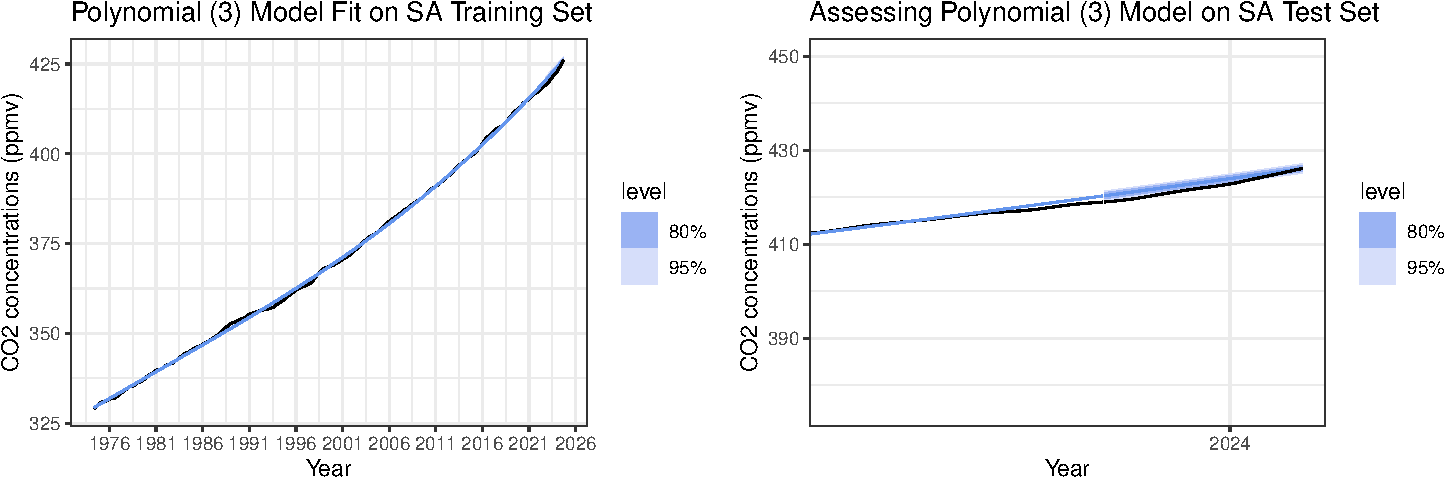
\includegraphics[width=1\linewidth]{lab_prompt_Updated_files/figure-latex/SA-poly-model-1} 

}

\caption{Assessing Polynomia (3) Model on SA data}\label{fig:SA-poly-model}
\end{figure}

We can see that Polynomial (3) model seems to fit the overall trend decently, although it does not perform so well on the forecast, with the actual data out of the 95\% confidence interval. The Polynomial (3) model also yielded a RMSE and MAE of 0.519 and 0.402 respectively for the training set, and a RMSE and MAE of 1.12 and 1.04 respectively for the test set. Although the ARIMA model outperformed the Polynomial (3) model by far on the training sets, the Polynomial (3) model did better with a lower RMSE and MAE on the test set.

\subsection{(3 points) Task Part 6b: How bad could it get?}\label{points-task-part-6b-how-bad-could-it-get}

With the non-seasonally adjusted data series, generate predictions for when atmospheric CO2 is expected to be at 420 ppm and 500 ppm levels for the first and final times (consider prediction intervals as well as point estimates in your answer). Generate a prediction for atmospheric CO2 levels in the year 2122. How confident are you that these will be accurate predictions?

\begin{Shaded}
\begin{Highlighting}[]
\CommentTok{\# Define a function to get the closest value}
\NormalTok{get\_closest }\OtherTok{\textless{}{-}} \ControlFlowTok{function}\NormalTok{(target, values) \{}
\NormalTok{  values[}\FunctionTok{which.min}\NormalTok{(}\FunctionTok{abs}\NormalTok{(values }\SpecialCharTok{{-}}\NormalTok{ target))]}
\NormalTok{\}}

\CommentTok{\# get first and last values}
\NormalTok{last\_420 }\OtherTok{\textless{}{-}} \FunctionTok{c}\NormalTok{(ci\_lower\_420[}\FunctionTok{length}\NormalTok{(ci\_lower\_420)], ci\_upper\_420[}\FunctionTok{length}\NormalTok{(ci\_upper\_420)])}
\NormalTok{last\_500 }\OtherTok{\textless{}{-}} \FunctionTok{c}\NormalTok{(ci\_lower\_500[}\FunctionTok{length}\NormalTok{(ci\_lower\_500)], ci\_upper\_500[}\FunctionTok{length}\NormalTok{(ci\_upper\_500)])}

\CommentTok{\# Find the closest .mean values in forecast\_df to each target in last\_420}
\NormalTok{closest\_420 }\OtherTok{\textless{}{-}} \FunctionTok{sapply}\NormalTok{(last\_420, get\_closest, }\AttributeTok{values =}\NormalTok{ forecast\_df}\SpecialCharTok{$}\NormalTok{.mean)}

\CommentTok{\# Filter forecast\_df for the closest .mean values for 420 ppm}
\NormalTok{matching\_dates\_420 }\OtherTok{\textless{}{-}}\NormalTok{ forecast\_df }\SpecialCharTok{\%\textgreater{}\%}
  \FunctionTok{filter}\NormalTok{(.mean }\SpecialCharTok{\%in\%}\NormalTok{ closest\_420) }\SpecialCharTok{\%\textgreater{}\%}
\NormalTok{  dplyr}\SpecialCharTok{::}\FunctionTok{select}\NormalTok{(monthyear, .mean)}

\CommentTok{\# Find the closest .mean values in forecast\_df to each target in last\_500}
\NormalTok{closest\_500 }\OtherTok{\textless{}{-}} \FunctionTok{sapply}\NormalTok{(last\_500, get\_closest, }\AttributeTok{values =}\NormalTok{ forecast\_df}\SpecialCharTok{$}\NormalTok{.mean)}

\CommentTok{\# Filter forecast\_df for the closest .mean values for 500 ppm}
\NormalTok{matching\_dates\_500 }\OtherTok{\textless{}{-}}\NormalTok{ forecast\_df }\SpecialCharTok{\%\textgreater{}\%}
  \FunctionTok{filter}\NormalTok{(.mean }\SpecialCharTok{\%in\%}\NormalTok{ closest\_500) }\SpecialCharTok{\%\textgreater{}\%}
\NormalTok{  dplyr}\SpecialCharTok{::}\FunctionTok{select}\NormalTok{(monthyear, .mean)}

\CommentTok{\# \# Display the results}
\CommentTok{\# matching\_dates\_420}
\CommentTok{\# matching\_dates\_500}
\CommentTok{\# }
\CommentTok{\# \# Looking at confidence intervals for first and last time 420 and 500 level is reached}
\CommentTok{\# c(ci\_lower\_420[1],  ci\_upper\_420[1])}
\CommentTok{\# c(ci\_lower\_500[1],  ci\_upper\_500[1])}
\end{Highlighting}
\end{Shaded}

\textbackslash begin\{table\}{[}H{]}
\centering
\textbackslash caption\{(\#tab:forecast\_420\_500)CO2 Levels and Forecasted Times ARIMA NSA with 80\% Confidence Intervals\}
\centering
\fontsize{9}{11}\selectfont

\begin{tabular}[t]{l|l|l|l|l}
\hline
CO2.Level & First.Month & First.Value & Last.Month & Last.Value\\
\hline
420 ppm & 2022 Nov & 419.01 & 2024 Jul & 422.7\\
\hline
500 ppm & 2043 Jun & 468.6 & 2068 Dec & 532.9\\
\hline
\end{tabular}

\textbackslash end\{table\}

Our model also forecasts CO2 levels in the year 2122. Although these forecasts include a standard deviation, but these do not take into account the existing efforts to reduce global greenhouse gases, such as the global effort to achieve net-zero GHG emissions by transitioning away from gas-cars to EVs. Thus, since these are very human-activity dependent, it is unlikely to be super accurate.

\begin{table}[H]
\centering
\caption{(\#tab:forecast_2122)CO2 Forecasts in 2122}
\centering
\fontsize{9}{11}\selectfont
\begin{tabular}[t]{l|r|r}
\hline
Date & Value & SD\\
\hline
2121 Dec & 663.8 & 107.3\\
\hline
2122 Jan & 663.8 & 107.3\\
\hline
2122 Jan & 663.7 & 107.3\\
\hline
2122 Jan & 663.7 & 107.4\\
\hline
2122 Jan & 663.4 & 107.4\\
\hline
2122 Feb & 663.1 & 107.4\\
\hline
2122 Feb & 662.7 & 107.4\\
\hline
2122 Feb & 662.3 & 107.5\\
\hline
2122 Feb & 661.7 & 107.5\\
\hline
2122 Mar & 661.3 & 107.5\\
\hline
2122 Mar & 660.6 & 107.6\\
\hline
2122 Mar & 659.9 & 107.6\\
\hline
2122 Mar & 659.8 & 107.6\\
\hline
2122 Mar & 659.3 & 107.7\\
\hline
2122 Apr & 659.1 & 107.7\\
\hline
2122 Apr & 658.5 & 107.7\\
\hline
2122 Apr & 658.1 & 107.7\\
\hline
2122 Apr & 658.0 & 107.8\\
\hline
2122 May & 657.9 & 107.8\\
\hline
2122 May & 657.7 & 107.8\\
\hline
2122 May & 657.8 & 107.9\\
\hline
2122 May & 658.1 & 107.9\\
\hline
2122 Jun & 658.4 & 107.9\\
\hline
2122 Jun & 658.7 & 108.0\\
\hline
2122 Jun & 658.8 & 108.0\\
\hline
2122 Jun & 659.2 & 108.0\\
\hline
2122 Jun & 659.9 & 108.0\\
\hline
2122 Jul & 660.1 & 108.1\\
\hline
2122 Jul & 660.6 & 108.1\\
\hline
2122 Jul & 660.9 & 108.1\\
\hline
2122 Jul & 661.1 & 108.2\\
\hline
2122 Aug & 661.3 & 108.2\\
\hline
2122 Aug & 661.8 & 108.2\\
\hline
2122 Aug & 662.2 & 108.3\\
\hline
2122 Aug & 662.5 & 108.3\\
\hline
2122 Aug & 662.5 & 108.3\\
\hline
2122 Sep & 662.8 & 108.3\\
\hline
2122 Sep & 663.2 & 108.4\\
\hline
2122 Sep & 663.5 & 108.4\\
\hline
2122 Sep & 663.4 & 108.4\\
\hline
2122 Oct & 663.6 & 108.5\\
\hline
2122 Oct & 663.7 & 108.5\\
\hline
2122 Oct & 664.0 & 108.5\\
\hline
2122 Oct & 663.8 & 108.5\\
\hline
2122 Nov & 664.0 & 108.6\\
\hline
2122 Nov & 664.3 & 108.6\\
\hline
2122 Nov & 664.9 & 108.6\\
\hline
2122 Nov & 665.6 & 108.7\\
\hline
2122 Nov & 665.7 & 108.7\\
\hline
2122 Dec & 665.7 & 108.7\\
\hline
2122 Dec & 665.9 & 108.8\\
\hline
2122 Dec & 666.0 & 108.8\\
\hline
2122 Dec & 666.2 & 108.8\\
\hline
\end{tabular}
\end{table}

\end{document}
